\renewcommand{\figurename}{}
\mychapter{R304 Services d'annuaires (10h30)}{cap:r304}
\lhead{R304 Services d'annuaires (10h30h)}

\vspace*{0.2cm}%
      \large
      \href{\@orientadorPagina}{\color{black}Enseignant\\Mr. Laurent Billon}\\%
\vspace*{0.5cm}%

Nous avons étudié lors de la première période à l'IUT les services d'annuaires. Ces services sont utilisés partout pour identifier les usagers et les assigner à des comptes utilisateurs. Extrêmement pratiques pour la gestion des utilisateurs, de leur droits et pour l'organisation générale d'une entreprise. Ceux-ci permettent un contrôle des accès unique pour les utilisateurs - plus besoin de renseigner un utilisateur à la main pour chaque service, plus besoin de renseigner énormément d'accès à l'arrivée ou au départ d'un nouveau membre : tout est synchronisé avec l'annuaire (les droits, les groupes, les utilisateurs...). Un serveur d'annuaire est un élément essentiel dans une organisation, qu'on doit savoir gérer. 

\section{Service d'annuaire LDAP}

Pour prendre en main les services d'annuaire, après un cours théorique il nous était demandé de monter un annuaire LDAP \textit{Lightweight Directory Access Protocol}. Toutes les commandes étaient données, le but de l'exercice était de comprendre l'organisation d'un annuaire pour répondre aux questions.
\\ \\
\begin{figure}[h]
    \centering
    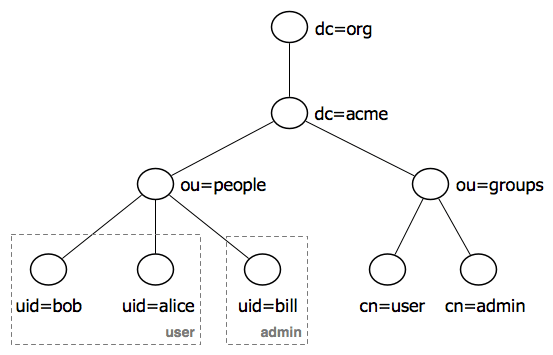
\includegraphics[width=1\linewidth]{imgs/acme_ldap.png}
    \caption{Schéma représentatif d'une hiérachie dans un annuaire}
    \label{fig:canal}
\end{figure}\\ \\
Un annuaire s'applique à un ou plusieurs DC \textit{Domain Component}, qui peuvent être un nom de domaine, un nom symbolique (e.g. DC = UPPA, ou DC = fr puis ce DC est rattaché à DC = univ-pau). Les DC sont la racine de l'arbre auquel vous souhaitez effectuer une recherche ou faire une affectation. 
\\ \\
À la suite de ces DC sont attachés des OU \textit{Organization Unit}, des groupes d'objets dans l'annuaire. Un exemple pourrait être la présence d'un OU pour les personnes de l'entreprise, puis dedans un OU \textit{Techniciens}, un OU \textit{Administrateurs}... L'agencement de l'arborescence se fait selon le besoin.
\\ \\
Ces OU sont composés de CN \textit{Common Name} qui sont les feuilles de l'arbre, l'élément final. Généralement des utilisateurs, des comptes... Peuvent aussi y être des UID \textit{User ID} pour globalement le même rôle, dépendemment de l'utilisation et des besoins.
\\ \\
Nous avons donc monté un serveur LDAP sous recommendations de l'enseignant pour ensuite monter l'arborescence voulue à l'aide de fichiers LDIF \textit{LDAP Data Interchange Format}. La recherche, l'ajout, la suppression ou la modificiation d'objet dans l'arbre se fait via l'écriture de fichiers LDIF, donnant une suite d'instruction à effectuer dans l'arbre.

\section{Aboutissants du module}

Par ce module nous avons appris comment monter un serveur LDAP, le gérer et par conséquence le comprendre. C'est un savoir essentiel en entreprise car extrêmement étant un outil largement présent et puissant.